
\documentclass[letterpaper,hide notes,xcolor={table,svgnames},pdftex,10pt]{beamer}
\def\showexamples{t}


%\usepackage[svgnames]{xcolor}

%% Demo talk
%\documentclass[letterpaper,notes=show]{beamer}

\usecolortheme{crane}
\setbeamertemplate{navigation symbols}{}

\usetheme{MyPittsburgh}
%\usetheme{Frankfurt}

%\usepackage{tipa}

\usepackage{hyperref}
\usepackage{graphicx,xspace}
\usepackage[normalem]{ulem}
\usepackage{multicol}
\usepackage{amsmath,amssymb,amsthm,graphicx,xspace}
\newcommand\SF[1]{$\bigstar$\footnote{SF: #1}}

\usepackage[default]{sourcesanspro}
\usepackage[T1]{fontenc}
\usepackage[scaled]{beramono}
\usepackage{tikzpagenodes}

\newcounter{tmpnumSlide}
\newcounter{tmpnumNote}


% old question code
%\newcommand\question[1]{{$\bigstar$ \small \onlySlide{2}{#1}}}
% \newcommand\nquestion[1]{\ifdefined \presentationonly \textcircled{?} \fi \note{\par{\Large \textbf{?}} #1}}
% \newcommand\nanswer[1]{\note{\par{\Large \textbf{A}} #1}}


 \newcommand\mnote[1]{%
   \addtocounter{tmpnumSlide}{1}
   \ifdefined\showcues {~\tiny\fbox{\arabic{tmpnumSlide}}}\fi
   \note{\setlength{\parskip}{1ex}\addtocounter{tmpnumNote}{1}\textbf{\Large \arabic{tmpnumNote}:} {#1\par}}}

\newcommand\mmnote[1]{\note{\setlength{\parskip}{1ex}#1\par}}

%\newcommand\mnote[2][]{\ifdefined\handoutwithnotes {~\tiny\fbox{#1}}\fi
% \note{\setlength{\parskip}{1ex}\textbf{\Large #1:} #2\par}}

%\newcommand\mnote[2][]{{\tiny\fbox{#1}} \note{\setlength{\parskip}{1ex}\textbf{\Large #1:} #2\par}}

\newcommand\mquestion[2]{{~\color{red}\fbox{?}}\note{\setlength{\parskip}{1ex}\par{\Large \textbf{?}} #1} \note{\setlength{\parskip}{1ex}\par{\Large \textbf{A}} #2\par}\ifdefined \presentationonly \pause \fi}

\newcommand\blackboard[1]{%
\ifdefined   \showblackboard
  {#1}
  \else {\begin{center} \fbox{\colorbox{blue!30}{%
         \begin{minipage}{.95\linewidth}%
           \hspace{\stretch{1}} Some space intentionally left blank; done at the blackboard.%
         \end{minipage}}}\end{center}}%
         \fi%
}



%\newcommand\q{\tikz \node[thick,color=black,shape=circle]{?};}
%\newcommand\q{\ifdefined \presentationonly \textcircled{?} \fi}

\usepackage{listings}
\lstset{basicstyle=\footnotesize\ttfamily,
	breaklines=true,
	aboveskip=15pt,
  	belowskip=15pt,
	frame=lines,
	numbers=left, basicstyle=\scriptsize, numberstyle=\tiny, stepnumber=0, numbersep=2pt
}

\usepackage{siunitx}
\newcommand\sius[1]{\num[group-separator = {,}]{#1}\si{\micro\second}}
\newcommand\sims[1]{\num[group-separator = {,}]{#1}\si{\milli\second}}
\newcommand\sins[1]{\num[group-separator = {,}]{#1}\si{\nano\second}}
\sisetup{group-separator = {,}, group-digits = true}

%% -------------------- tikz --------------------
\usepackage{tikz}
\usetikzlibrary{positioning}
\usetikzlibrary{arrows,backgrounds,automata,decorations.shapes,decorations.pathmorphing,decorations.markings,decorations.text,decorations.pathreplacing}

\tikzstyle{place}=[circle,draw=blue!50,fill=blue!20,thick, inner sep=0pt,minimum size=6mm]
\tikzstyle{transition}=[rectangle,draw=black!50,fill=black!20,thick, inner sep=0pt,minimum size=4mm]

\tikzstyle{block}=[rectangle,draw=black, thick, inner sep=5pt]
\tikzstyle{bullet}=[circle,draw=black, fill=black, thin, inner sep=2pt]

\tikzstyle{pre}=[<-,shorten <=1pt,>=stealth',semithick]
\tikzstyle{post}=[->,shorten >=1pt,>=stealth',semithick]
\tikzstyle{bi}=[<->,shorten >=1pt,shorten <=1pt, >=stealth',semithick]

\tikzstyle{mut}=[-,>=stealth',semithick]

\tikzstyle{treereset}=[dashed,->, shorten >=1pt,>=stealth',thin]

\usepackage{ifmtarg}
\usepackage{xifthen}
\makeatletter
% new counter to now which frame it is within the sequence
\newcounter{multiframecounter}
% initialize buffer for previously used frame title
\gdef\lastframetitle{\textit{undefined}}
% new environment for a multi-frame
\newenvironment{multiframe}[1][]{%
\ifthenelse{\isempty{#1}}{%
% if no frame title was set via optional parameter,
% only increase sequence counter by 1
\addtocounter{multiframecounter}{1}%
}{%
% new frame title has been provided, thus
% reset sequence counter to 1 and buffer frame title for later use
\setcounter{multiframecounter}{1}%
\gdef\lastframetitle{#1}%
}%
% start conventional frame environment and
% automatically set frame title followed by sequence counter
\begin{frame}%
\frametitle{\lastframetitle~{\normalfont(\arabic{multiframecounter})}}%
}{%
\end{frame}%
}
\makeatother

\makeatletter
\newdimen\tu@tmpa%
\newdimen\ydiffl%
\newdimen\xdiffl%
\newcommand\ydiff[2]{%
    \coordinate (tmpnamea) at (#1);%
    \coordinate (tmpnameb) at (#2);%
    \pgfextracty{\tu@tmpa}{\pgfpointanchor{tmpnamea}{center}}%
    \pgfextracty{\ydiffl}{\pgfpointanchor{tmpnameb}{center}}%
    \advance\ydiffl by -\tu@tmpa%
}
\newcommand\xdiff[2]{%
    \coordinate (tmpnamea) at (#1);%
    \coordinate (tmpnameb) at (#2);%
    \pgfextractx{\tu@tmpa}{\pgfpointanchor{tmpnamea}{center}}%
    \pgfextractx{\xdiffl}{\pgfpointanchor{tmpnameb}{center}}%
    \advance\xdiffl by -\tu@tmpa%
}
\makeatother
\newcommand{\copyrightbox}[3][r]{%
\begin{tikzpicture}%
\node[inner sep=0pt,minimum size=2em](ciimage){#2};
\usefont{OT1}{phv}{n}{n}\fontsize{4}{4}\selectfont
\ydiff{ciimage.south}{ciimage.north}
\xdiff{ciimage.west}{ciimage.east}
\ifthenelse{\equal{#1}{r}}{%
\node[inner sep=0pt,right=1ex of ciimage.south east,anchor=north west,rotate=90]%
{\raggedleft\color{black!50}\parbox{\the\ydiffl}{\raggedright{}#3}};%
}{%
\ifthenelse{\equal{#1}{l}}{%
\node[inner sep=0pt,right=1ex of ciimage.south west,anchor=south west,rotate=90]%
{\raggedleft\color{black!50}\parbox{\the\ydiffl}{\raggedright{}#3}};%
}{%
\node[inner sep=0pt,below=1ex of ciimage.south west,anchor=north west]%
{\raggedleft\color{black!50}\parbox{\the\xdiffl}{\raggedright{}#3}};%
}
}
\end{tikzpicture}
}


%% --------------------

%\usepackage[excludeor]{everyhook}
%\PushPreHook{par}{\setbox0=\lastbox\llap{MUH}}\box0}

%\vspace*{\stretch{1}

%\setbox0=\lastbox \llap{\textbullet\enskip}\box0}

\setlength{\parskip}{\fill}

\newcommand\noskips{\setlength{\parskip}{1ex}}
\newcommand\doskips{\setlength{\parskip}{\fill}}

\newcommand\xx{\par\vspace*{\stretch{1}}\par}
\newcommand\xxs{\par\vspace*{2ex}\par}
\newcommand\tuple[1]{\langle #1 \rangle}
\newcommand\code[1]{{\sf \footnotesize #1}}
\newcommand\ex[1]{\uline{Example:} \ifdefined \presentationonly \pause \fi
  \ifdefined\showexamples#1\xspace\else{\uline{\hspace*{2cm}}}\fi}

\newcommand\ceil[1]{\lceil #1 \rceil}


\AtBeginSection[]
{
   \begin{frame}
       \frametitle{Outline}
       \tableofcontents[currentsection]
   \end{frame}
}



\pgfdeclarelayer{edgelayer}
\pgfdeclarelayer{nodelayer}
\pgfsetlayers{edgelayer,nodelayer,main}

\tikzstyle{none}=[inner sep=0pt]
\tikzstyle{rn}=[circle,fill=Red,draw=Black,line width=0.8 pt]
\tikzstyle{gn}=[circle,fill=Lime,draw=Black,line width=0.8 pt]
\tikzstyle{yn}=[circle,fill=Yellow,draw=Black,line width=0.8 pt]
\tikzstyle{empty}=[circle,fill=White,draw=Black]
\tikzstyle{bw} = [rectangle, draw, fill=blue!20, 
    text width=4em, text centered, rounded corners, minimum height=2em]
    
    \newcommand{\CcNote}[1]{% longname
	This work is licensed under the \textit{Creative Commons #1 3.0 License}.%
}
\newcommand{\CcImageBy}[1]{%
	\includegraphics[scale=#1]{creative_commons/cc_by_30.pdf}%
}
\newcommand{\CcImageSa}[1]{%
	\includegraphics[scale=#1]{creative_commons/cc_sa_30.pdf}%
}
\newcommand{\CcImageNc}[1]{%
	\includegraphics[scale=#1]{creative_commons/cc_nc_30.pdf}%
}
\newcommand{\CcGroupBySa}[2]{% zoom, gap
	\CcImageBy{#1}\hspace*{#2}\CcImageNc{#1}\hspace*{#2}\CcImageSa{#1}%
}
\newcommand{\CcLongnameByNcSa}{Attribution-NonCommercial-ShareAlike}

\newenvironment{changemargin}[1]{% 
  \begin{list}{}{% 
    \setlength{\topsep}{0pt}% 
    \setlength{\leftmargin}{#1}% 
    \setlength{\rightmargin}{1em}
    \setlength{\listparindent}{\parindent}% 
    \setlength{\itemindent}{\parindent}% 
    \setlength{\parsep}{\parskip}% 
  }% 
  \item[]}{\end{list}} 




\title{Lecture 2 --- Modern Processors }

\author{Jeff Zarnett \\ \small \texttt{jzarnett@uwaterloo.ca}}
\institute{Department of Electrical and Computer Engineering \\
  University of Waterloo}
\date{\today}


\begin{document}

\begin{frame}
  \titlepage

\end{frame}



\begin{frame}
\frametitle{Modern Processors}


Remember the classic von Neumann machine architecture. 

A program is comprised of both instructions and data, both of which are stored in the same memory. 

A program executes sequentially, one statement at a time, one after another.

 That is not really how computers work, at least not anymore, but it is an abstraction we still maybe find useful when it comes to algorithm analysis.

\end{frame}



\begin{frame}
\frametitle{CPU Frequency Over Time}


\begin{center}
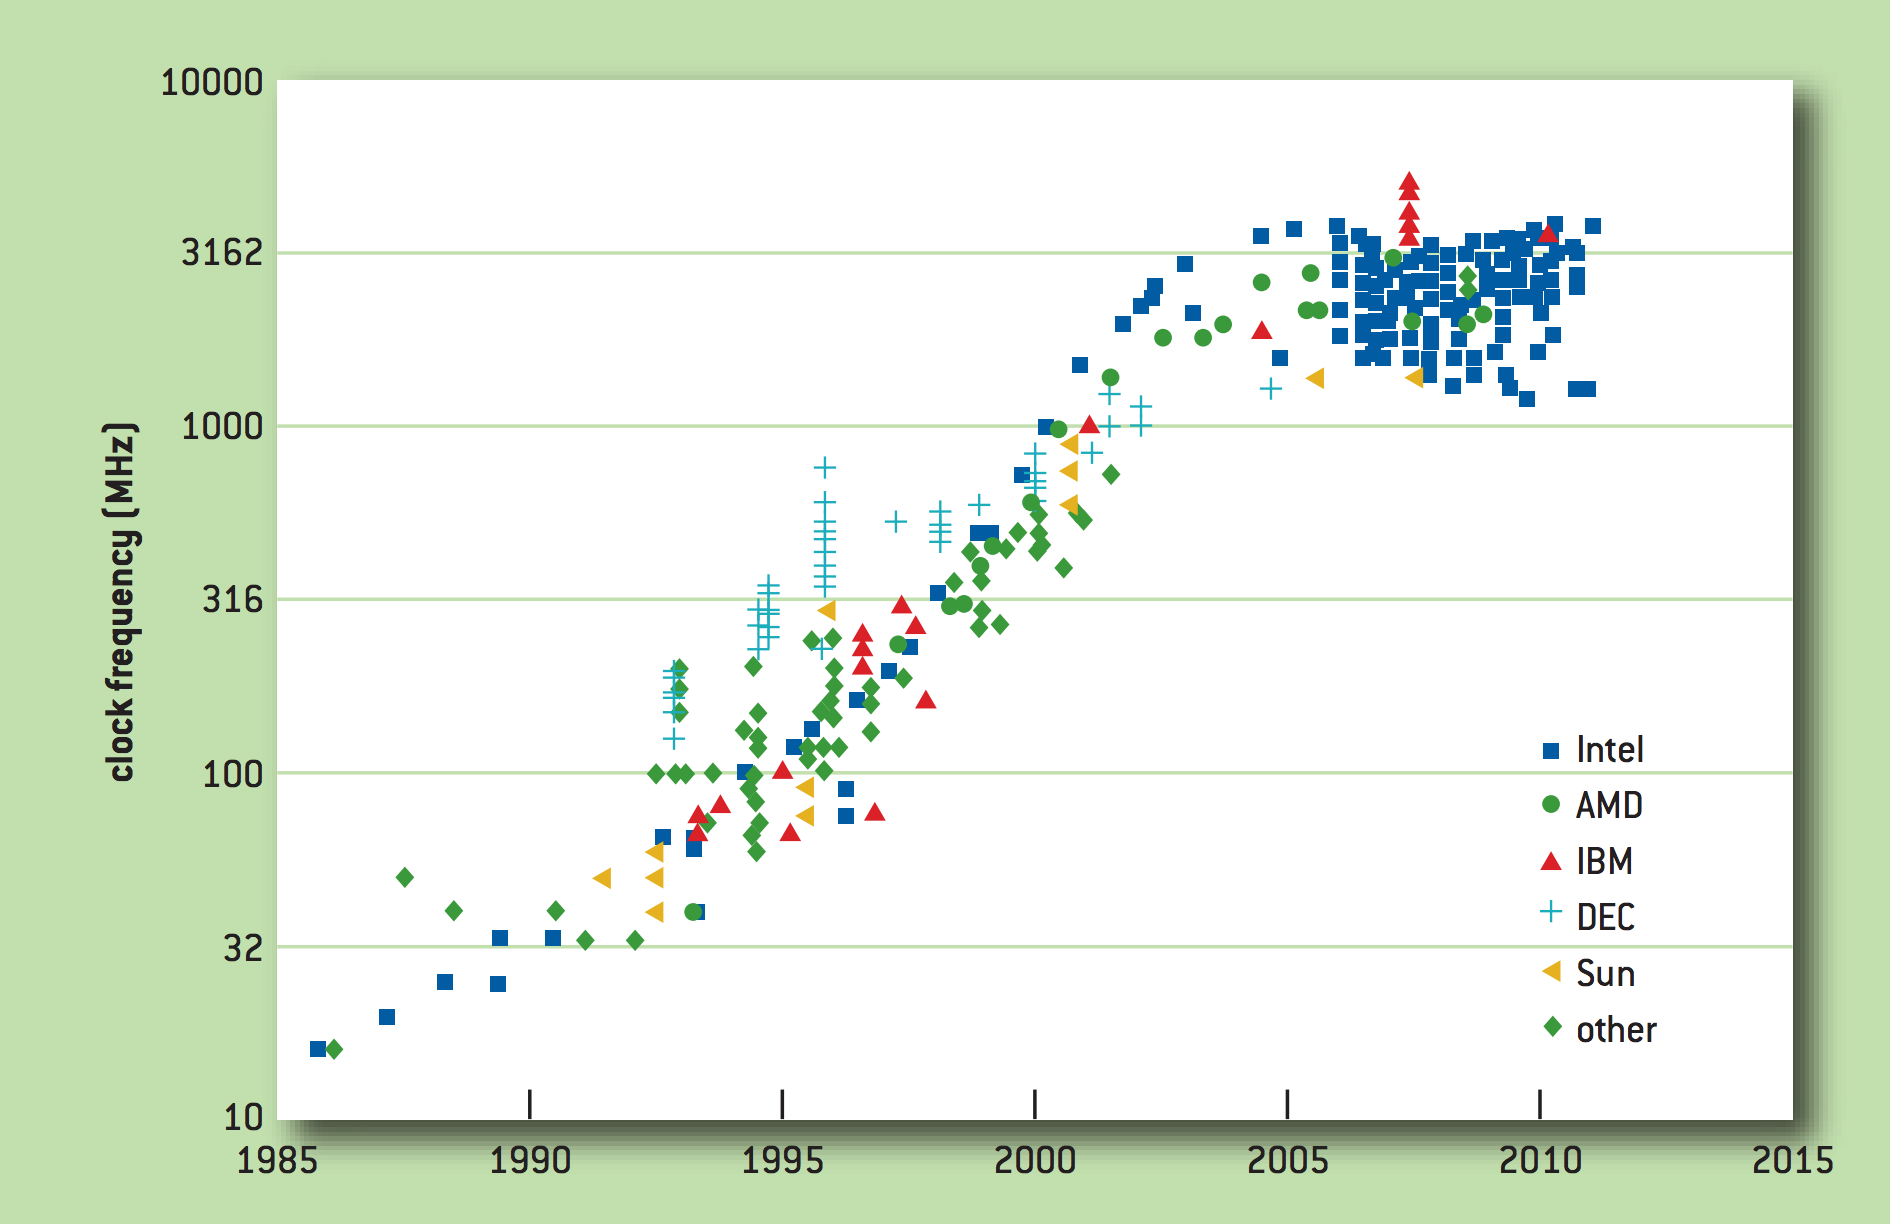
\includegraphics[width=\textwidth]{images/cpu-frequency}
\end{center}

\end{frame}



\begin{frame}
\frametitle{CPU Frequency Over Time}

The x86 processor is a Complex Instruction Set Computing (CISC) processor.\\
\quad In other words, there are a lot of assembly instructions. 

But why? This was intended for your convenience as a programmer!

So the hardware people thought they were doing everyone a favour. 

These are easy to program in, from the way the assembly programmer thinks, but hard to implement and hard to pipeline. 

\end{frame}



\begin{frame}
\frametitle{CISC}

For a lot of CISC machines, the Cycles Per Instruction (CPI) varied, something like 4-10 cycles to complete any instruction, but at least it was predictable. 

Program performance was basically the number of page faults times the amount of time it takes to read from disk, plus the instruction execution time.

Thus the optimization goal is: minimize page faults. 

Page fault count is relatively easy to measure and there are some things we can do to reduce the number of page faults.

If you were working with an embedded system with no disk (or at least no page faults) then the optimization goal is minimize instruction count.

\end{frame}



\begin{frame}
\frametitle{RISCy Business}

Between 1990 and 2005 we got some impressive scaling on CPU frequency.

We got Reduced Instruction Set Computing (RISC) CPUs. 

Simpler processors are easier to scale than complex ones, and simpler instructions mean fewer cycles per instruction.

That also means we can have more pipelining.

 The tradeoff is that RISC CPUs are much harder to program in assembly directly, so compilers had to do the work. 
 
\end{frame}



\begin{frame}
\frametitle{RISCy Business}

Consider delay slots: an instruction after a branch is always executed or worse, the result of a computation is not available to the next instruction. 

In these cases the ``simple'' solution is to put a \texttt{NOP} (do-nothing) instruction in.

Good compilers (and programmers) can rearrange instructions, hopefully, to make this work without wasting time. 

Also: memory got cheaper, so we have more of it, so page faults occurred less and less frequently.


\end{frame}


\begin{frame}
\frametitle{Over The Wall}

But then, as we have seen, we hit the (power) wall. 

And you might think, well, if I run into a wall, I can just go around it.\\
\quad There must be other ways to advance! 

And there are, except, we hit three other walls too, and now we are surrounded.

What are these other three seemingly-insurmountable barriers?

\end{frame}

\begin{frame}
\frametitle{Mr. Gorbachev, Tear Down This Wall!}
\begin{center}
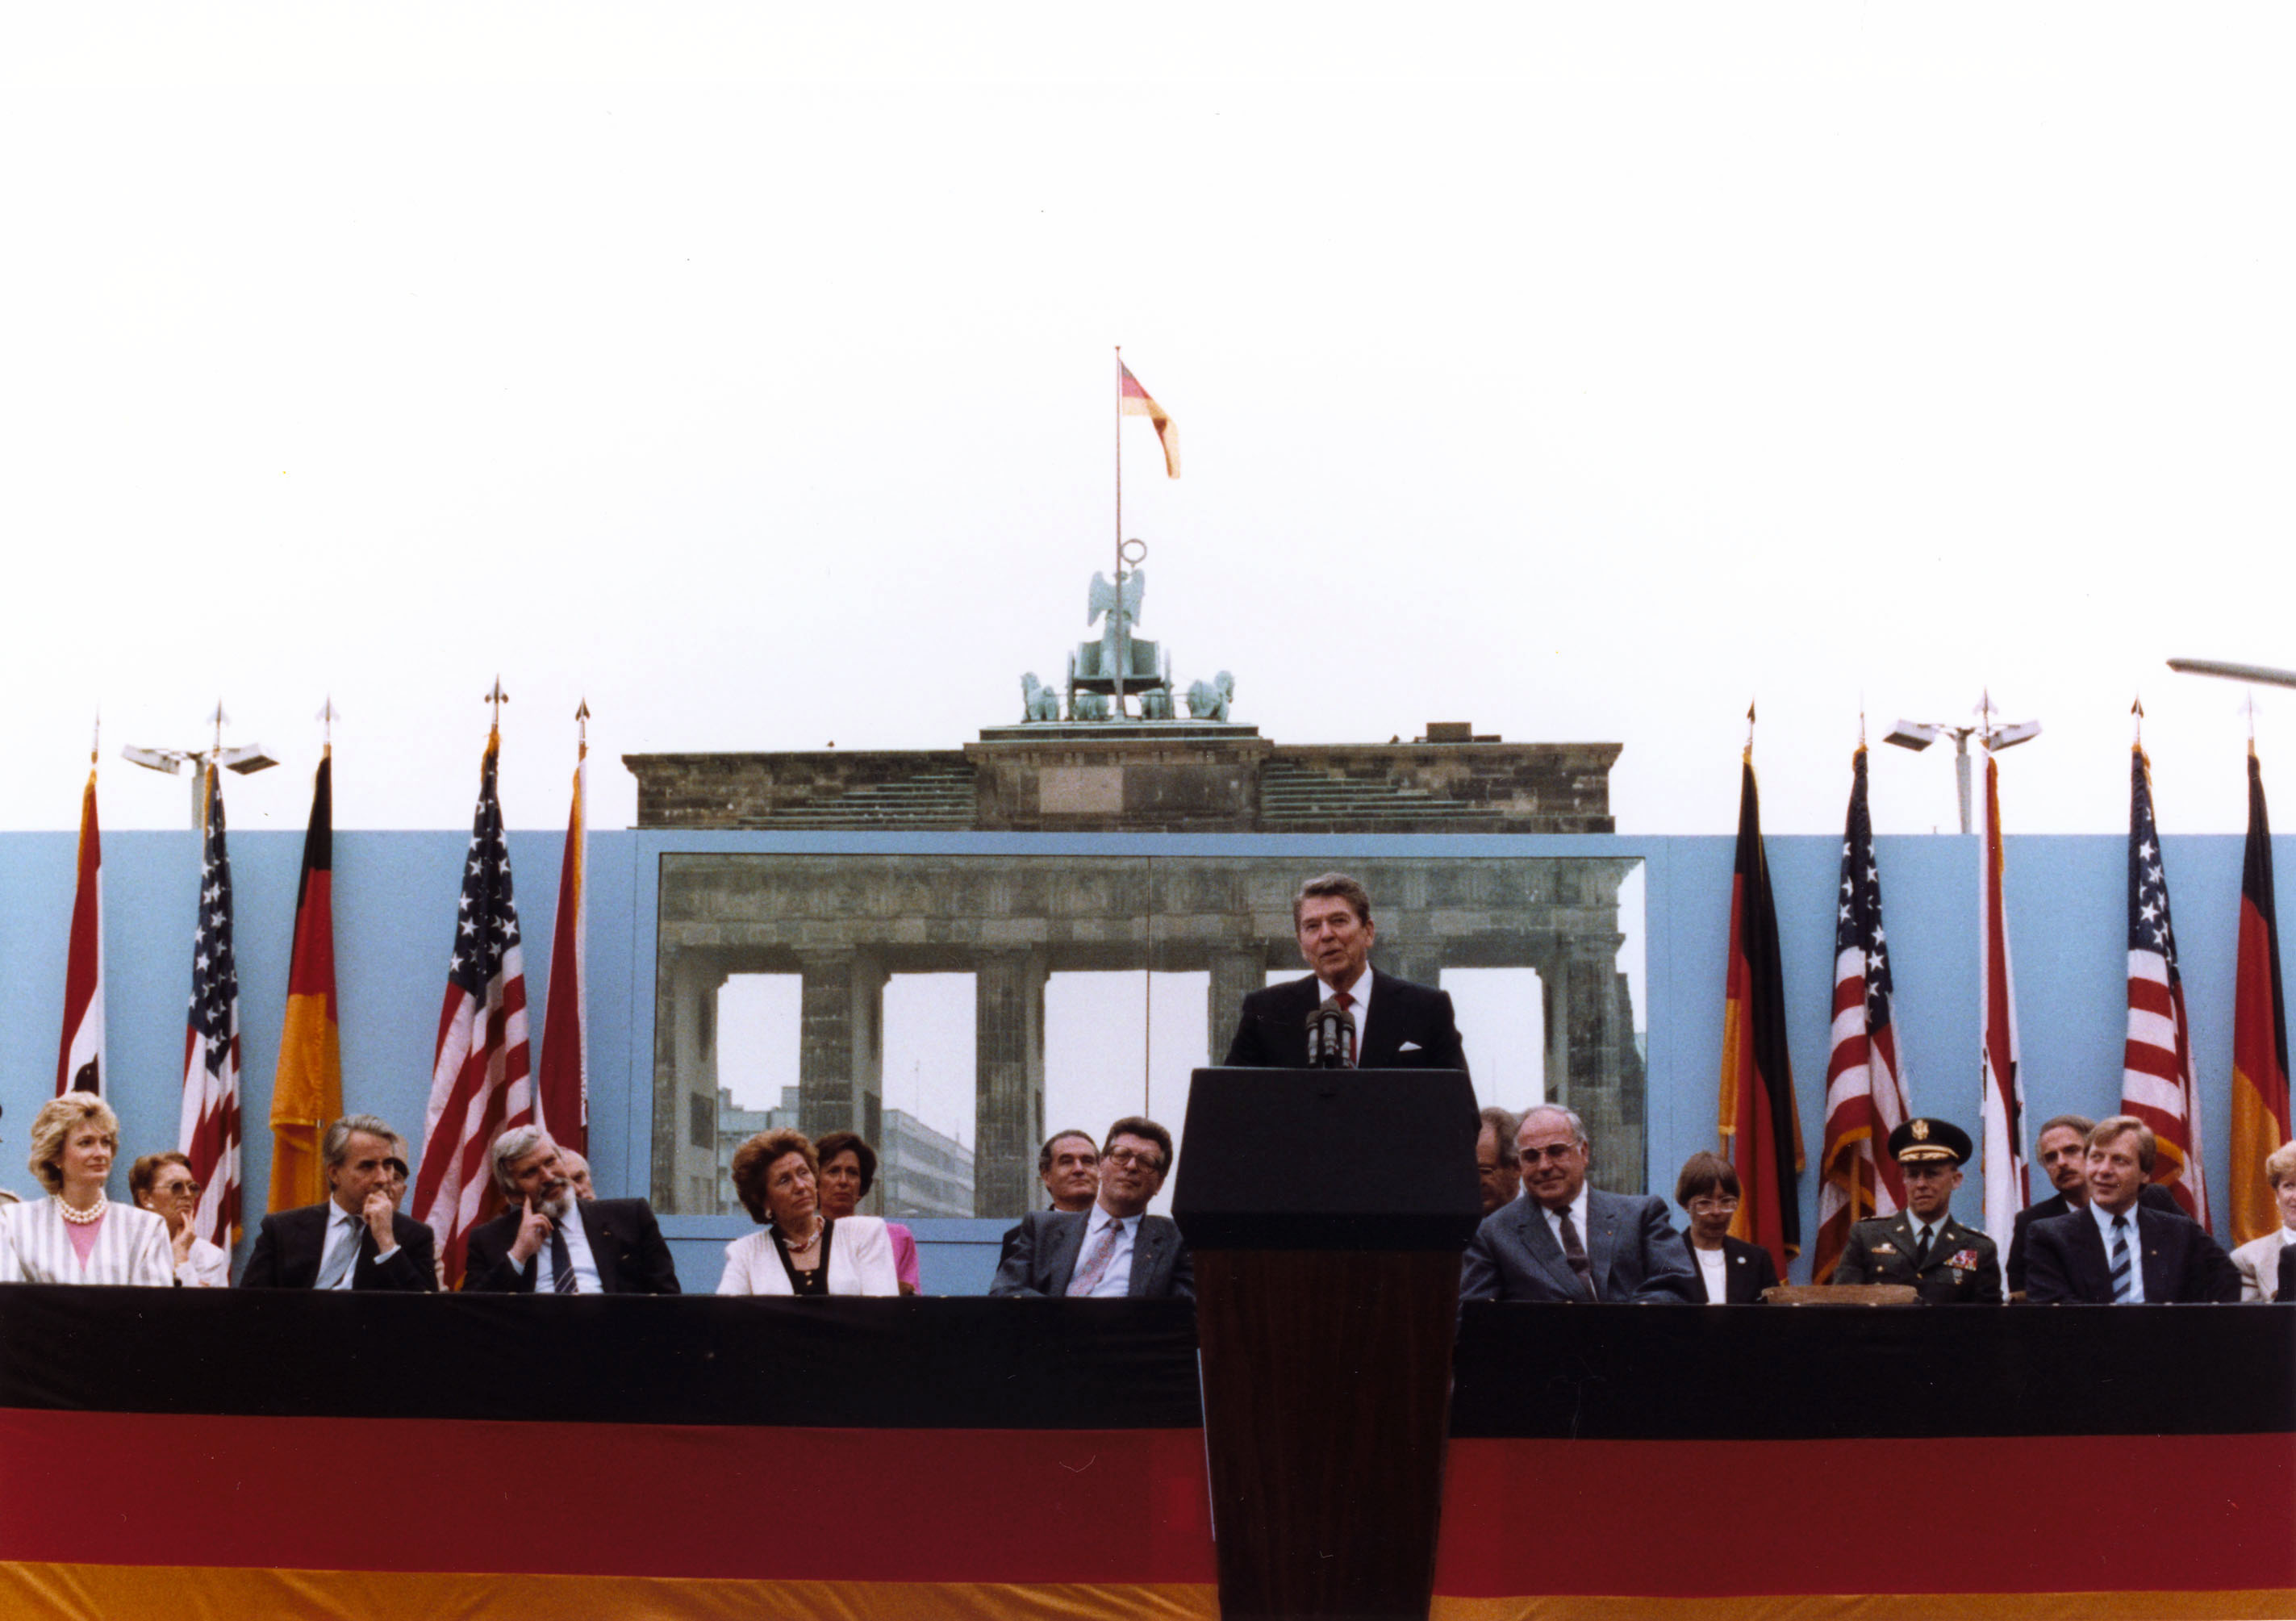
\includegraphics[width=\textwidth]{images/ReaganBerlinWall.jpg}
\end{center}
\end{frame}


\begin{frame}
\frametitle{Mr. Gorbachev, Tear Down This Wall!}

Instruction level parallelism (ILP) is getting close to the limit of what we can do. 

We can predict branches with a certain accuracy but if we have already got 95\% efficiency, our maximum improvement is 5\%.

The speed of memory advances has not kept up with the advances in CPUs. 

So now we have moved from the era of runtime being dominated by page faults to the era of runtime being dominated by cache misses. 

Doubling, say, level one cache (at great expense) does not double the speed of the program; it may speed it up by a small amount at most. 

\end{frame}



\begin{frame}
\frametitle{Quicker Than a Ray of Light}

\begin{center}
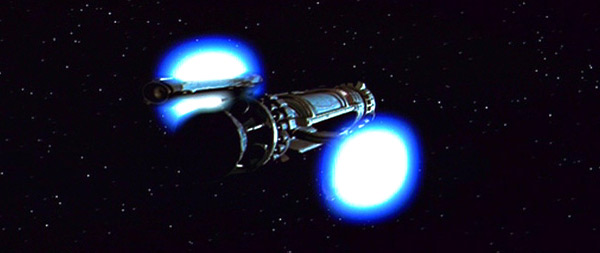
\includegraphics[width=.8\textwidth]{images/L02-phoenix-warp}\\
{\scriptsize \hfill Memory Alpha, Phoenix goes to Warp, ST:FC}
\end{center}

The final wall is the universal speed limit: the speed of light.

 The more complex the CPU is, the longer the path any signal may have to travel to get from A to B. 
 
 This is limited, most practically, by the speed of light, and thus far, nobody has invented a way to get around this universal speed limit.
\end{frame}



\begin{frame}
\frametitle{Back to ILP}

The idea with ILP is not having more cycles to work with, but instead, doing more in each clock cycle. And there's a lot of clever ideas. 

Pipelining: you may have heard a bit about his already, especially so if you have (or are currently) taking a CPU architecture course.
\end{frame}



\begin{frame}
\frametitle{Pipelining}

To complete an instruction there are five basic steps:
\begin{enumerate}
\item Fetch the instruction from memory
\item Decode the instruction
\item Fetch needed operands
\item Perform the operation, and 
\item Write the result
\end{enumerate}

Example: \texttt{ADD R1, R2}


\end{frame}



\begin{frame}
\frametitle{Pipelining}

Thus even a simple instruction takes more than one clock cycle, but the good news is that the stages can overlap:

\begin{center}
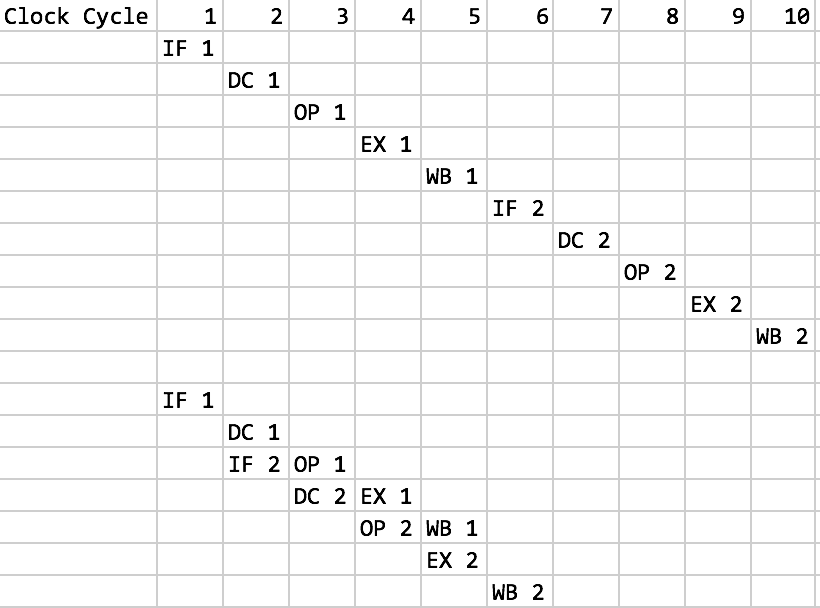
\includegraphics[width=0.8\textwidth]{images/pipelining}
\end{center}

\end{frame}


\begin{frame}
\frametitle{Hazard Lights}

There are pipeline hazards: sometimes you need the result of a previous step before you can go on. 

These prevent us from reaching the theoretical maximum of one instruction completed per clock cycle. 

There are other hazards; we may have conflicts over certain CPU resources or fetch may be unable to identify the next instruction because of a branch. 

In the worst case, if we've mispredicted a branch, we have to flush the pipeline. 

In that case, some extra work was done that was not necessary\ldots 

\end{frame}



\begin{frame}
\frametitle{Fetch Quest!}

If we do a load from memory, and we are lucky, it is found in the fastest cache and is available in perhaps 2-3 clock cycles. 

If we must go to memory, it may be 200-300 cycles. 

If it is in level 2 or level 3 cache it will be somewhere in between. 

The key idea, though, is if we are trying to put something in register \texttt{R7}, it will take time until that value is actually present in that register. 

The simplest approach is to just wait around until that value has arrived, and then go on to the next instruction. 

That works, but we can do better.

\end{frame}



\begin{frame}
\frametitle{Shadow of Mordor}

That better idea is: continue executing until \texttt{R7} is used somewhere. 

This allows us to get some useful work done in the meantime. 

Hardware keeps track of the fact that the register is not quite ready yet, but the work can get done in what is called the ``miss shadow''. 

It's possible to have more than one load in flight at a time, two or more can be done in various CPU architectures, but it is of course hardware dependant. 

\end{frame}



\begin{frame}
\frametitle{Branch Prediction}

Branch prediction has come up already, but if we have a load followed by a compare used as a branch, we can then, well, guess. 

If we are wrong, there is the need to cleanup. But the good news is that branch prediction is usually right most of the time, perhaps 95\% or more.

\end{frame}



\begin{frame}
\frametitle{Dual Issue}

Another nice thing that the hardware can do for us is ``dual issue'' instructions. 

If we have two consecutive instructions that both take the same amount of time, use unrelated registers, and don't consume two of the same resource.

Example: \texttt{ADD R1, 16} and \texttt{CMP R2, 0}. 

In an embedded system, you may be interested in ensuring that this happens during a computationally intensive loop, such as encoding/decoding of media. 

If programmed correctly, you can be sure you get dual issue on every cycle.


\end{frame}




\begin{frame}
\frametitle{A Trio}

Then a group of things that somewhat go together: register renaming, branch prediction, speculation, and Out-of-Order (O-O-O) Execution. 

Register renaming works on a fairly simple principle: an assembly instruction says to read from register \texttt{R4}. 

Behind the scenes inside the processor, it is mapped to a physical register (let's say \texttt{RA} for the purpose of the example).


\end{frame}



\begin{frame}[fragile]
\frametitle{Register Renaming}

Consider the following assembly instructions:

\begin{verbatim}
MOV R2, R7 + 32
ADD R1, R2
MOV R2, R9 + 64
ADD R3, R2
\end{verbatim}

\end{frame}




\begin{frame}
\frametitle{Branch Prediction Synergy}

This has a certain synergy with the branch prediction. 

If we predict a branch, we can do speculative changes into one set of registers while we keep the ``old'' register values around too. 

When we figure out whether the branch prediction is correct, we can then get rid of the ones we don't need.

So we get better recovery if there is a misprediction.

\end{frame}



\begin{frame}[fragile]
\frametitle{It ain't about how hard you hit\ldots}

Most importantly, it allows us to get past a cache miss and keep going.

The goal here is to run until we can start the next cache miss, because the sooner that starts the sooner it's over, and the faster the program executes.


\begin{verbatim}
ld rax, rbx+16
add rbx, 16
cmp rax, 0
jeq null_chk
st rbx-16, rcx
ld rcx, rdx
ld rax, rax+8
\end{verbatim}


\end{frame}



\begin{frame}
\frametitle{It's about how hard you can get hit \& keep moving forward}

There are seven operations we were trying to do here with two cache misses. 

The cache misses complete in cycles 300 and 304 (maybe 302 if we have dual issue), so in total we complete 7 operations in about 305 cycles. 

All the trickery and cleverness got us to that second miss which means we complete in 305. 

If we did not manage that, it would take about 600 cycles to complete it all. 

So we did double performance, even though in this example our overall performance was very, very low.

\end{frame}



\begin{frame}
\frametitle{Intel Itanium}

For years Intel was trying to push its Itanium processors. 

The goal of these was to find static (compile-time) parallelism: if a machine has infinite registers, can speculate infinitely, etc, the program gets sped up. 

Run all possibilities in parallel and at the end figure out which is right.

Unfortunately it didn't work out very well because this requires the right kind of program and an super smart compiler. 

Oh yes, and infinite registers requires infinite space as well as infinite money. 

So instead the quest has turned to how to get better performance out of x86\ldots

\end{frame}



\begin{frame}
\frametitle{x86 Instead}

The x86 approach tries to maximize dynamic (run-time) parallelism. 

This has been done incrementally, with more pipelining, re-order buffers, adding more functional units, and so on. 

Cache miss rates and branch mispredicts continue to dominate performance, even though the rates are very low, because a miss costs so much. 

\end{frame}



\begin{frame}
\frametitle{Moore's Law\ldots}

Something like 90-99\% of the transistors on a modern x86 chip are spent in cache. 

In spite of the extreme complexity of the decode logic that allows multiple parallel decodes of all the weird and wacky instructions of the x86\ldots

Pushing cache to the biggest size it can be is so important because it prevents the performance hit of going to memory.


\end{frame}



\begin{frame}
\frametitle{Bad Trend}

The image below (from Sun World Wide Analyst Conference in 2003) is obviously a bit dated and rather insulting:
\begin{center}
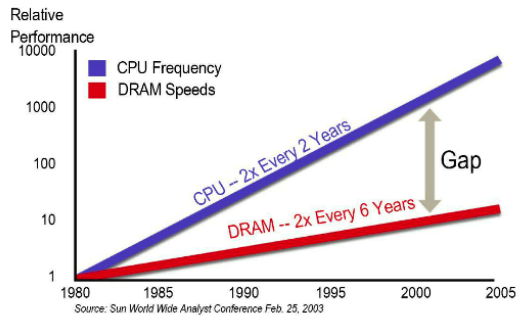
\includegraphics[width=0.6\textwidth]{images/ram-vs-cpu.png}
\end{center}

\end{frame}



\begin{frame}
\frametitle{RAM Types}

DRAM is, however, not the only kind of memory. 

There is SRAM (Static RAM) which is fast but expensive, the kind of stuff that goes on the CPU die, and it is six transistors per bit. 

Compare against DRAM which is much cheaper, but slow: one transistor and one capacitor per bit. 

Improvements in DRAM have not really improved latency but have improved bandwidth. 

DDR means there are two transfers per cycle, but it still takes significant time to get any data out. 

And DRAM needs occasional refreshes (capacitors\ldots) so sometimes we have to wait for that.

\end{frame}



\begin{frame}
\frametitle{Disk?!}

In the Operating Systems course you probably learned that disk is the slowest thing and the limiting factor. 

That's true, as Obi-Wan Kenobi would say, from a certain point of view. 

Now that we live in the world of Solid State Drives (SSDs), ``disk'' reads are about as fast as memory reads and memory reads are the rate-limiting step. 

More is the new more, orange is the new black, and memory is the new disk.

\end{frame}



\begin{frame}
\frametitle{Future Ideas}

To get memory access speed up there are things we can do, like relax coherency constraints, more synchronization through locks\ldots 

All of which we will come back to in some upcoming lectures. 

If we want to get better performance, we need to figure out where time is going. 

For that we will have the subject of profiling, which comes up later.

If we can track down where our cache misses are occurring, maybe, just maybe, we can do something about it. 


\end{frame}


\begin{frame}
\frametitle{Modern Processors}

If you'd much prefer to hear this material from someone else, the source for this lecture is:

\begin{center}
\url{http://www.infoq.com/presentations/click-crash-course-modern-hardware}
\end{center}

\end{frame}

\begin{frame}
\frametitle{Cache Misses}

As discussed, the CPU generates a memory address for a read or write operation.

The address will be mapped to a page. 

Ideally, the page is found in the cache.\\
\quad If it is, we call it a \alert{cache hit};\\
\quad Otherwise, it is a \alert{cache miss}.

\end{frame}



\begin{frame}
\frametitle{Missed Me by THIS Much}

Miss: we must load the page from memory, a comparatively slow operation.


The \%age of the time that a page is found in the cache is called the \alert{hit ratio}.

 The effective access time is therefore computed as:

\begin{center}
Effective Access Time = $h \times t_{c} + (1-h) \times t_{m}$
\end{center}

\end{frame}



\begin{frame}
\frametitle{Cache Size - How Much can you Afford?}

Intel 64-bit CPUs tend to have L1, L2, and L3 caches. 

L1 is the smallest and L3 is the largest.

\begin{center}
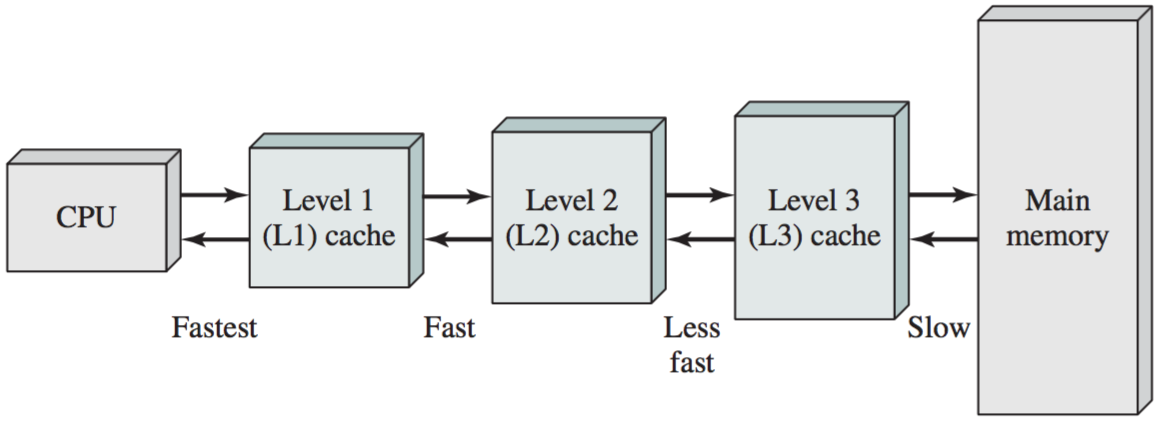
\includegraphics[width=0.6\textwidth]{images/caches.png}\\
Three levels of cache between the CPU and main memory.
\end{center}


\end{frame}



\begin{frame}
\frametitle{Pay Up}

Cliff Click said that 5\% miss rates dominate performance. Let's look at why.

Here are the reported cache miss rates for SPEC CPU2006.

\begin{center}
\begin{tabular}{ll}
L1D & 40 per 1000 \\
L2 & 4 per 1000
\end{tabular}
\end{center}

Let's assume that the L1D cache miss penalty is 5 cycles and the L2 miss penalty is
300 cycles, as in the video. 

Then, for every instruction, you would expect a running
time of, on average:
\[ 1 + 0.04 \times 5 + 0.004 \times 300 = 2.4. \]

\end{frame}



\begin{frame}
\frametitle{Bring in the Disk}

If we replace the terms $t_{c}$ and $t_{m}$ with $t_{m}$ and $t_{d}$ (time to retrieve it from disk) respectively, and redefine $h$ as $p$, the chance that a page is in memory.

Effective access time in virtual memory: 

\begin{center}
	Effective Access Time = $ p \times t_{m} + (1 - p) \times t_{d}$
\end{center}


\end{frame}



\begin{frame}
\frametitle{Put It Together}

We can combine the caching and disk read formulae to get the true effective access time for a system where there is only 1 level of cache:

\begin{center}
	Effective Access Time = $ h \times t_{c} + (1 - h) ( p \times t_{m} + (1 - p) \times t_{d})$
\end{center}

We can measure $t_{d}$ if we're so inclined.

\end{frame}



\begin{frame}
\frametitle{Slow as A Snail Chained to an Anvil}

The slow step is the amount of time it takes to load the page from disk. 

A typical hard drive may have a latency of 3~ms, seek time is around 5~ms, and a transfer time of 0.05~ms. 

This is  several orders of magnitude larger than any of the other costs.

Several requests may be queued, making the time even longer.

\end{frame}



\begin{frame}
\frametitle{Dominating Flurry}


Thus the disk read term $t_{d}$ dominates the effective access time equation. 

We can roughly estimate the access time in nanoseconds as $(1-p) \times 8~000~000$. 

If the page fault rate is high, performance is awful. If performance of the computer is to be reasonable, the page fault rate has to be very, very low. 


Summary: misses are not just expensive, they hurt performance the most.

\end{frame}


\end{document}

